\documentclass[12pt]{article}

\usepackage[margin=1in]{geometry}
\usepackage{amsmath, amssymb}
\usepackage{graphicx}
\usepackage{booktabs}
\usepackage{enumitem}
\usepackage{hyperref}
\usepackage{natbib}

\title{Risk-Appropriate Neonatal Care and Maternal Mental Health:
Evidence from Medicaid  (2016--2019) }

\author{
Mario Mart\'{\i}nez-Jim\'enez\thanks{Imperial  Business School, Department of Economics \& Public Policy. Stanford University School of Medicine (Department of Health Policy).} Helen Kissel\thanks{Stanford University }
 
}

\date{\today}

\begin{document}
\maketitle

\begin{abstract}
We study whether delivering a clinically vulnerable newborn in a county with limited access to risk-appropriate neonatal intensive care is associated with worse maternal mental health outcomes. We link Medicaid Transformed Medicaid Statistical Information System Analytic Files (TAF) for 2016--2019 (good-quality states) to a hospital-level NICU registry with neonatal level-of-care designations and bed capacity, and construct residence-to-hospital travel distances to quantify geographic access. We define vulnerability using newborn diagnosis codes for prematurity and low birthweight, and measure maternal mental health using postpartum diagnoses, service use, and psychotropic medications in claims.

\vspace{0.5em}
\noindent \textbf{JEL codes:} I12, I18, J13\\
\textbf{Keywords:} NICU access; risk-appropriate care; prematurity; Medicaid; maternal mental health; geographic distance
\end{abstract}

\newpage

\section{Introduction}
Neonatal intensive care is organized around the concept of \emph{risk-appropriate care}: infants with higher clinical risk should be delivered in, or promptly transferred to, facilities with the personnel, equipment, and subspecialty services appropriate for their needs. Geographic variation in NICU capability and capacity implies that some mothers---especially those in rural or low-resource areas---may face longer travel, emergent neonatal transfers, and parent--infant separation when a vulnerable infant is delivered in a low-capability setting. We ask: \emph{Does limited local access to risk-appropriate NICU care worsen maternal postpartum mental health among Medicaid-covered births?}

cansee\section{Background: Levels of Neonatal Care in the U.S.}
NICU levels in the U.S., defined by the American Academy of Pediatrics (AAP), range from Level I (basic care for healthy newborns) to Level IV (highest, most critical care). Levels II--IV specialize in treating premature or ill infants, with Level IV providing the most complex, specialized, and around-the-clock care for infants requiring surgery or advanced, long-term care.

\subsection{AAP level definitions}
\begin{enumerate}[leftmargin=*, itemsep=0.25em]
  \item \textbf{Level I (Well-Baby Nursery):} Basic care for stable, healthy, full-term infants; routine newborn exams; stabilization for transfer; stabilization of near-term infants.
  \item \textbf{Level II (Special Care Nursery):} Care for infants born $\geq 32$ weeks gestation or weighing $\geq 1500$g who are moderately ill, recovering from serious illness, or requiring specialized care (e.g., IV antibiotics, feeding support, supplemental oxygen).
  \item \textbf{Level III (NICU):} Care for infants born $<32$ weeks, weighing $<1500$g, or requiring specialized services (e.g., sustained mechanical ventilation), with capability for some surgical procedures.
  \item \textbf{Level IV (Regional NICU):} Highest level of care for the most critically ill newborns, including complex surgical, cardiac, or respiratory needs; full range of pediatric subspecialists and advanced, 24/7 long-term support.
\end{enumerate}

\subsection{Capacity and utilization}
Recent evidence reports approximately 35,601 NICU beds nationally, with Level III beds comprising the largest share. NICU admission rates have increased over time, reaching 9.8\% of births by 2023, and rising from 8.7\% in 2016 to 9.3\% in 2019.

\section{Data}
\subsection{Medicaid claims (TAF), 2016--2019}
We use TAF enrollment and claims files for 2016--2019 from states meeting CMS/TAF quality criteria (``good-quality states''). The analytic unit is a Medicaid-covered delivery. We link maternal delivery episodes to infant records and follow mothers postpartum to observe mental health outcomes.

\subsection{NICU registry and hospital characteristics}
We compile a hospital-level registry with (i) county location (via geocoding), (ii) AAP-aligned NICU level (I--IV or equivalent state designation mapped to the AAP framework), and (iii) NICU bed counts (capacity). We aggregate hospital NICU supply to county-year measures such as:
\[
\texttt{BEDS}_{c,t}^{(L\geq 3)} = \sum_{h \in c} \texttt{BEDS}_{h,t}\cdot \mathbf{1}\{\texttt{LEVEL}_{h,t}\geq 3\}.
\]

\subsection{Infant vulnerability definitions (diagnosis codes)}
We define newborn vulnerability using infant diagnosis codes observed on the birth hospitalization and early neonatal claims.

\begin{center}
\begin{tabular}{l l}
\toprule
\textbf{Construct} & \textbf{Diagnosis codes (claims-based)} \\
\midrule
Preterm (ICD-10-CM) & \texttt{P07.2*} (extreme immaturity), \texttt{P07.3*} (preterm, 28--36 wks) \\
Low birthweight (ICD-10-CM) & \texttt{P07.0*} (extremely low BW), \texttt{P07.1*} (other low BW, 1000--2499g) \\
Preterm / LBW (ICD-9-CM) & \texttt{765.0x}, \texttt{765.1x} (BW-based), \texttt{765.2x} (gestational age) \\
\bottomrule
\end{tabular}
\end{center}

We also construct severity tiers (e.g., VLBW/ELBW; $<32$ weeks) using the more granular ICD-10 subcodes when available.

\subsection{Maternal mental health outcomes}
Maternal postpartum mental health is measured using three complementary claim-based outcomes:
(i) diagnoses (e.g., depression/anxiety, PTSD, SUD, self-harm),
(ii) service use (behavioral health visits, ED visits, inpatient psychiatric admissions),
and (iii) medication fills (e.g., antidepressants/anxiolytics/antipsychotics; NDC-based).

\section{Methods}

\subsection{Geographic access and travel distance}
Let $(\phi_i,\lambda_i)$ denote maternal residence latitude/longitude at delivery (ZIP centroid; fallback to county centroid), and $(\phi_h,\lambda_h)$ the delivery hospital coordinates. We compute great-circle distance using the haversine formula:
\[
d(i,h)=2R\arcsin\left(\sqrt{\sin^2\left(\frac{\phi_h-\phi_i}{2}\right)+
\cos(\phi_i)\cos(\phi_h)\sin^2\left(\frac{\lambda_h-\lambda_i}{2}\right)}\right),
\]
with earth radius $R\approx 6371$ km.

We construct:
\begin{itemize}[leftmargin=*, itemsep=0.25em]
  \item \texttt{dist\_res\_to\_delivery}\,: $d(i,h^{\text{del}})$.
  \item \texttt{dist\_res\_to\_nearest\_L3plus}\,: $\min_{h \in \mathcal{H}_{L\geq 3}} d(i,h)$.
  \item \texttt{no\_L3plus\_in\_county}\,: $\mathbf{1}\{\texttt{BEDS}_{c(i),t}^{(L\geq 3)}=0\}$.
  \item \texttt{excess\_distance}\,: $\texttt{dist\_res\_to\_delivery}-\texttt{dist\_res\_to\_nearest\_L3plus}$.
\end{itemize}

\subsection{Risk-appropriate care mismatch}
Let $\texttt{VULN}_i$ indicate an infant who is preterm and/or low birthweight (or meets a stricter tier such as $<32$ weeks or $<1500$g). Define a residence-based access indicator:
\[
\texttt{NO\_APPROPRIATE}_{c,t} = \mathbf{1}\{\texttt{BEDS}_{c,t}^{(L\geq 3)}=0\},
\]
and (optionally) a delivery-facility mismatch indicator:
\[
\texttt{MISMATCH}_i=\mathbf{1}\{\texttt{VULN}_i=1\}\cdot \mathbf{1}\{\texttt{LEVEL}_{h^{\text{del}}(i),t}<3\}.
\]

\subsection{Estimation}
Our baseline design estimates differential associations for vulnerable versus non-vulnerable births exposed to limited local access:
\begin{equation}
Y_{i}=\beta\,\big(\texttt{VULN}_{i}\times \texttt{NO\_APPROPRIATE}_{c(i),t(i)}\big)
+\gamma\,\texttt{VULN}_{i}
+\delta\,X_{i}
+\alpha_{c(i)}+\tau_{t(i)}+\varepsilon_{i},
\end{equation}
where $Y_i$ is a postpartum maternal mental health outcome, $X_i$ includes maternal demographics and pre-pregnancy mental health history, $\alpha_{c}$ are county fixed effects, and $\tau_{t}$ are time fixed effects (e.g., year-by-month). We extend the model to include distance-based exposure (\texttt{dist\_res\_to\_nearest\_L3plus}) and capacity measures (beds per birth) to capture both \emph{availability} and \emph{strain}.

\section{Results}
\subsection{Descriptive patterns}
We describe (i) geographic NICU location, (ii) facility counts by NICU level, and (iii) high-acuity bed capacity. All maps in this section are constructed from the NeonatologySolutions NICU directory (N=1,402 facilities). We classify facilities using the directory's reported \texttt{NICU Level}. For state-level counts, we count facilities in each state by level. For county-level counts, we assign facilities to counties using ZIP-to-county crosswalk matching and then count facilities by county. We report Level II separately and aggregate higher-acuity facilities as Level III+IV. Bed-capacity maps sum reported \texttt{Beds} across Level III and Level IV facilities within each state or county.

Map legends are binned from the underlying count/bed distributions, and the map annotations report the mean and standard deviation across all states (state maps) or all counties (county maps), including zeros. Alaska and Hawaii are repositioned for visualization.

\begin{figure}[htbp!]
\centering
\caption{NICU locations in the United States}
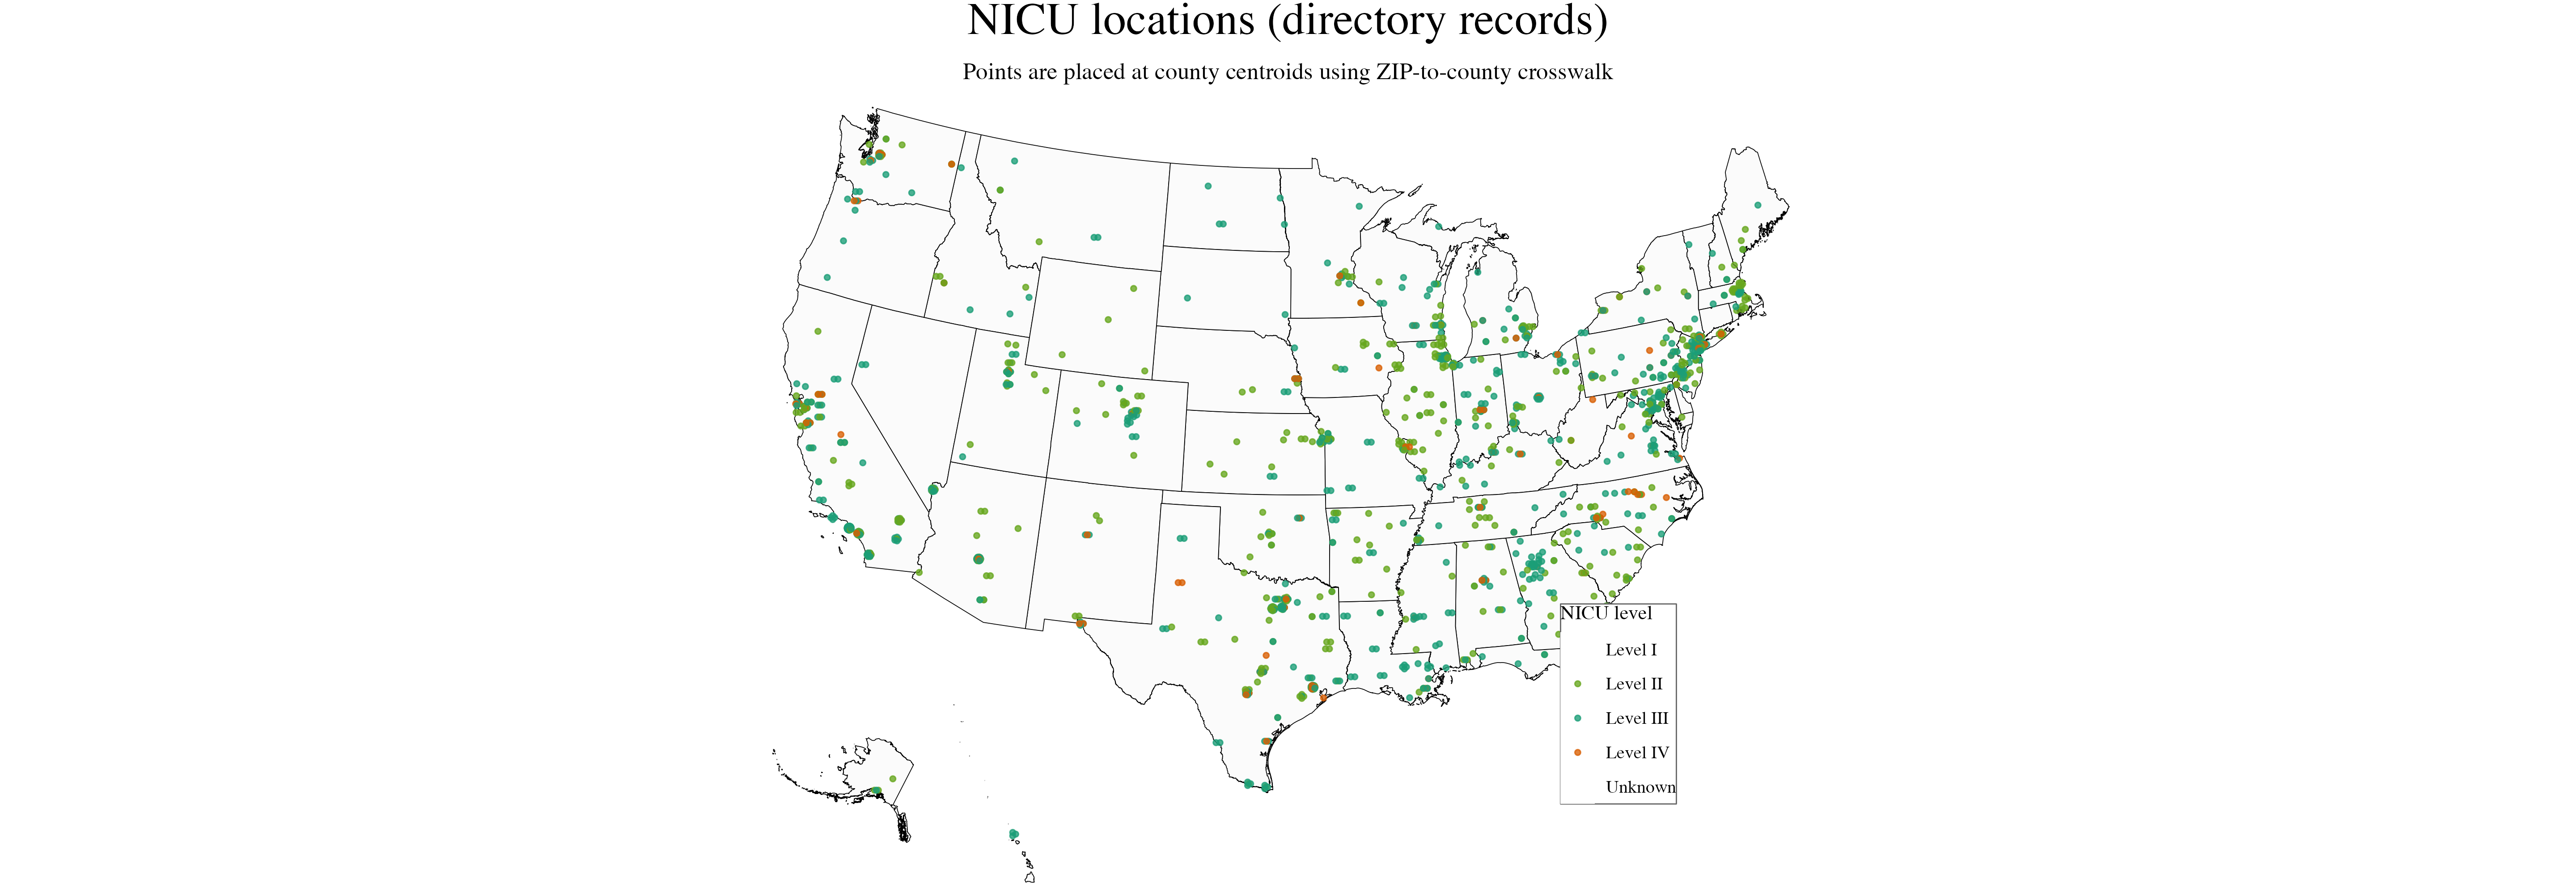
\includegraphics[width=\textwidth]{Figures/Background/nicu_locations.png}
\label{fig:nicu_locations}
\end{figure}

\begin{figure}[htbp!]
\centering
\caption{NICU Level II facility count by state}
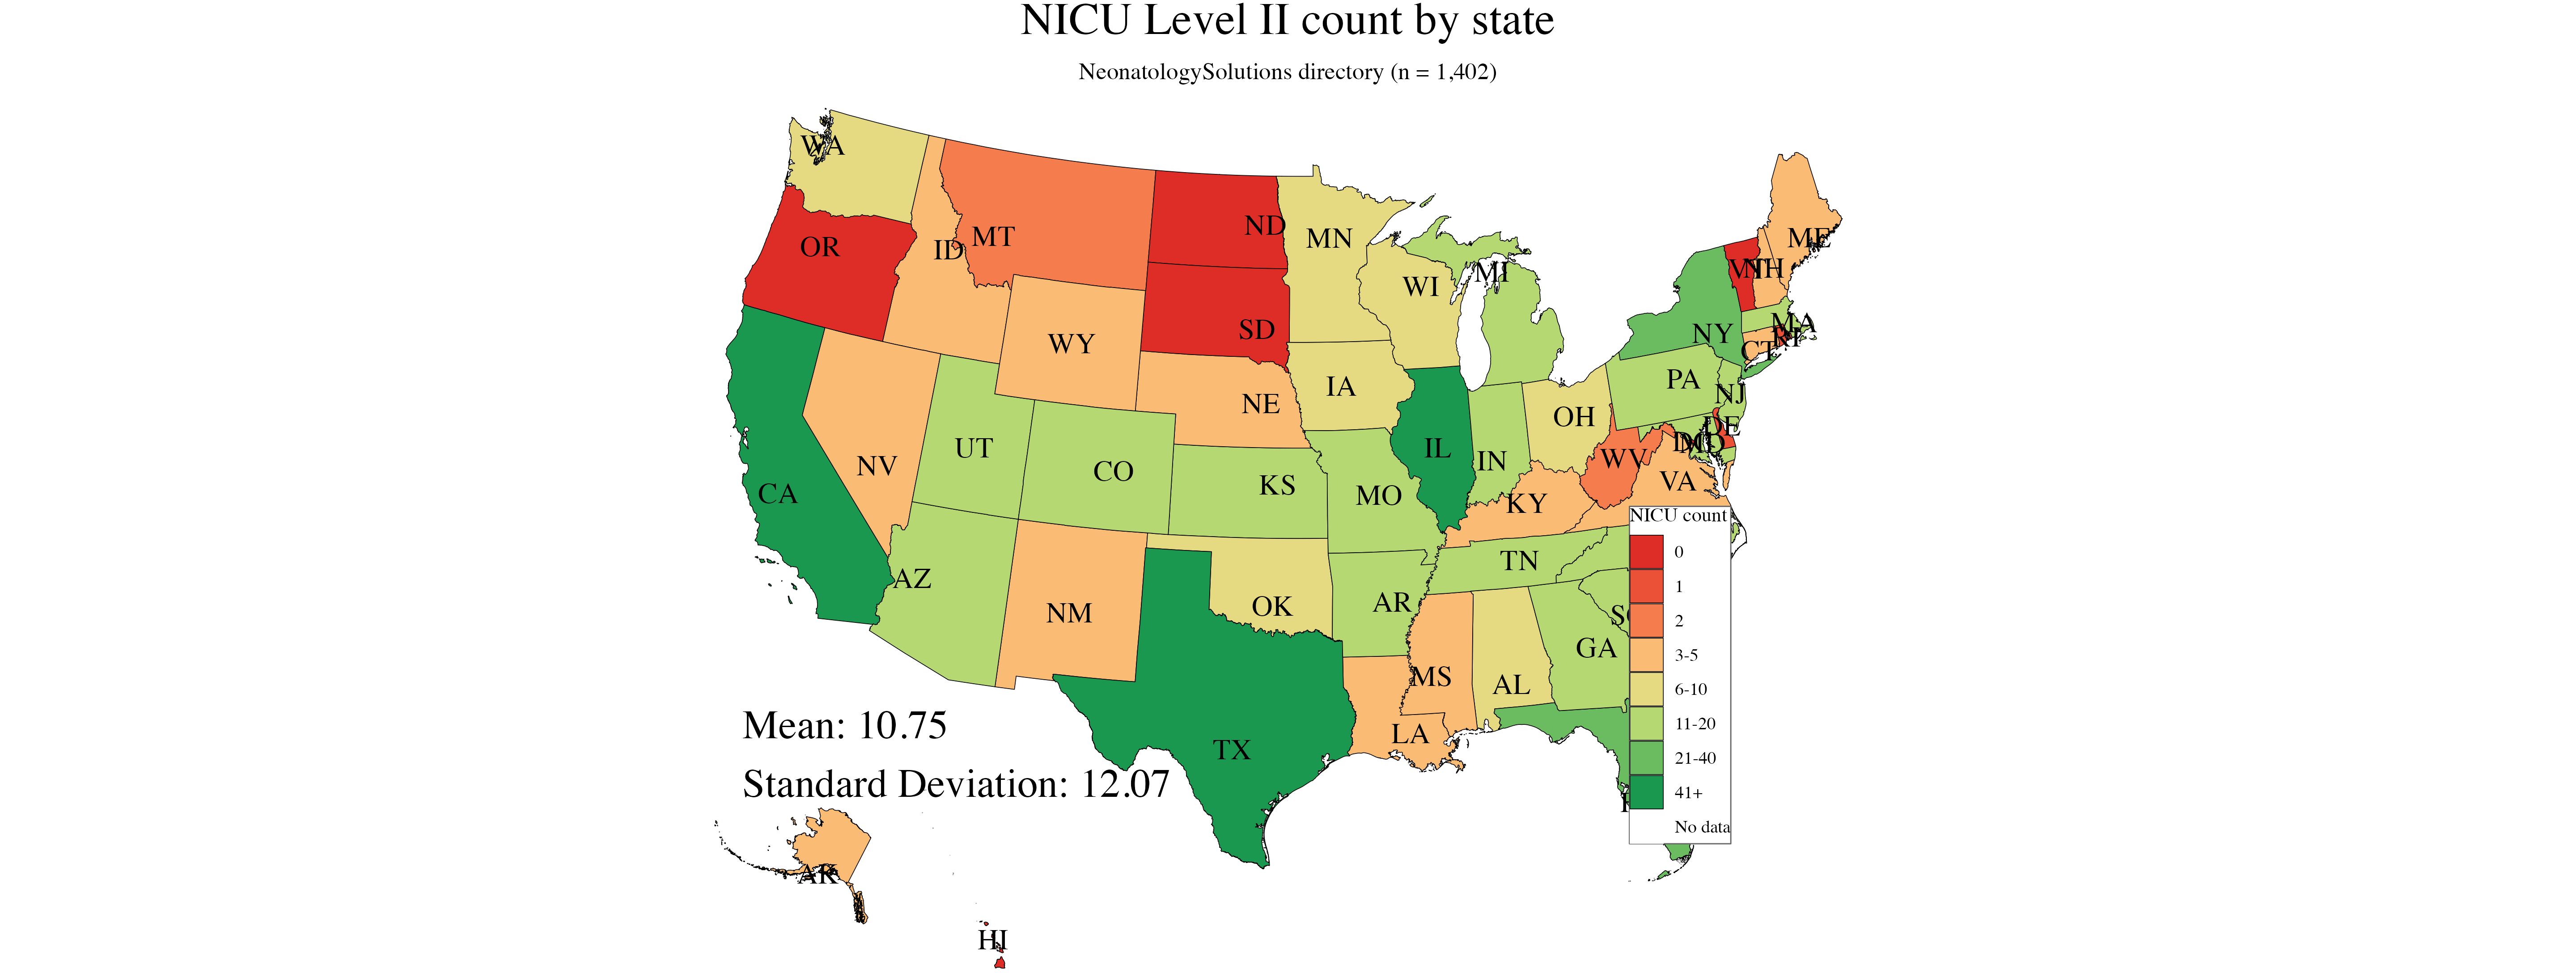
\includegraphics[width=\textwidth]{Figures/Background/nicu_state_level_II_count.png}
\label{fig:nicu_state_level2_count}
\end{figure}

\begin{figure}[htbp!]
\centering
\caption{NICU Level III + IV facility count by state}
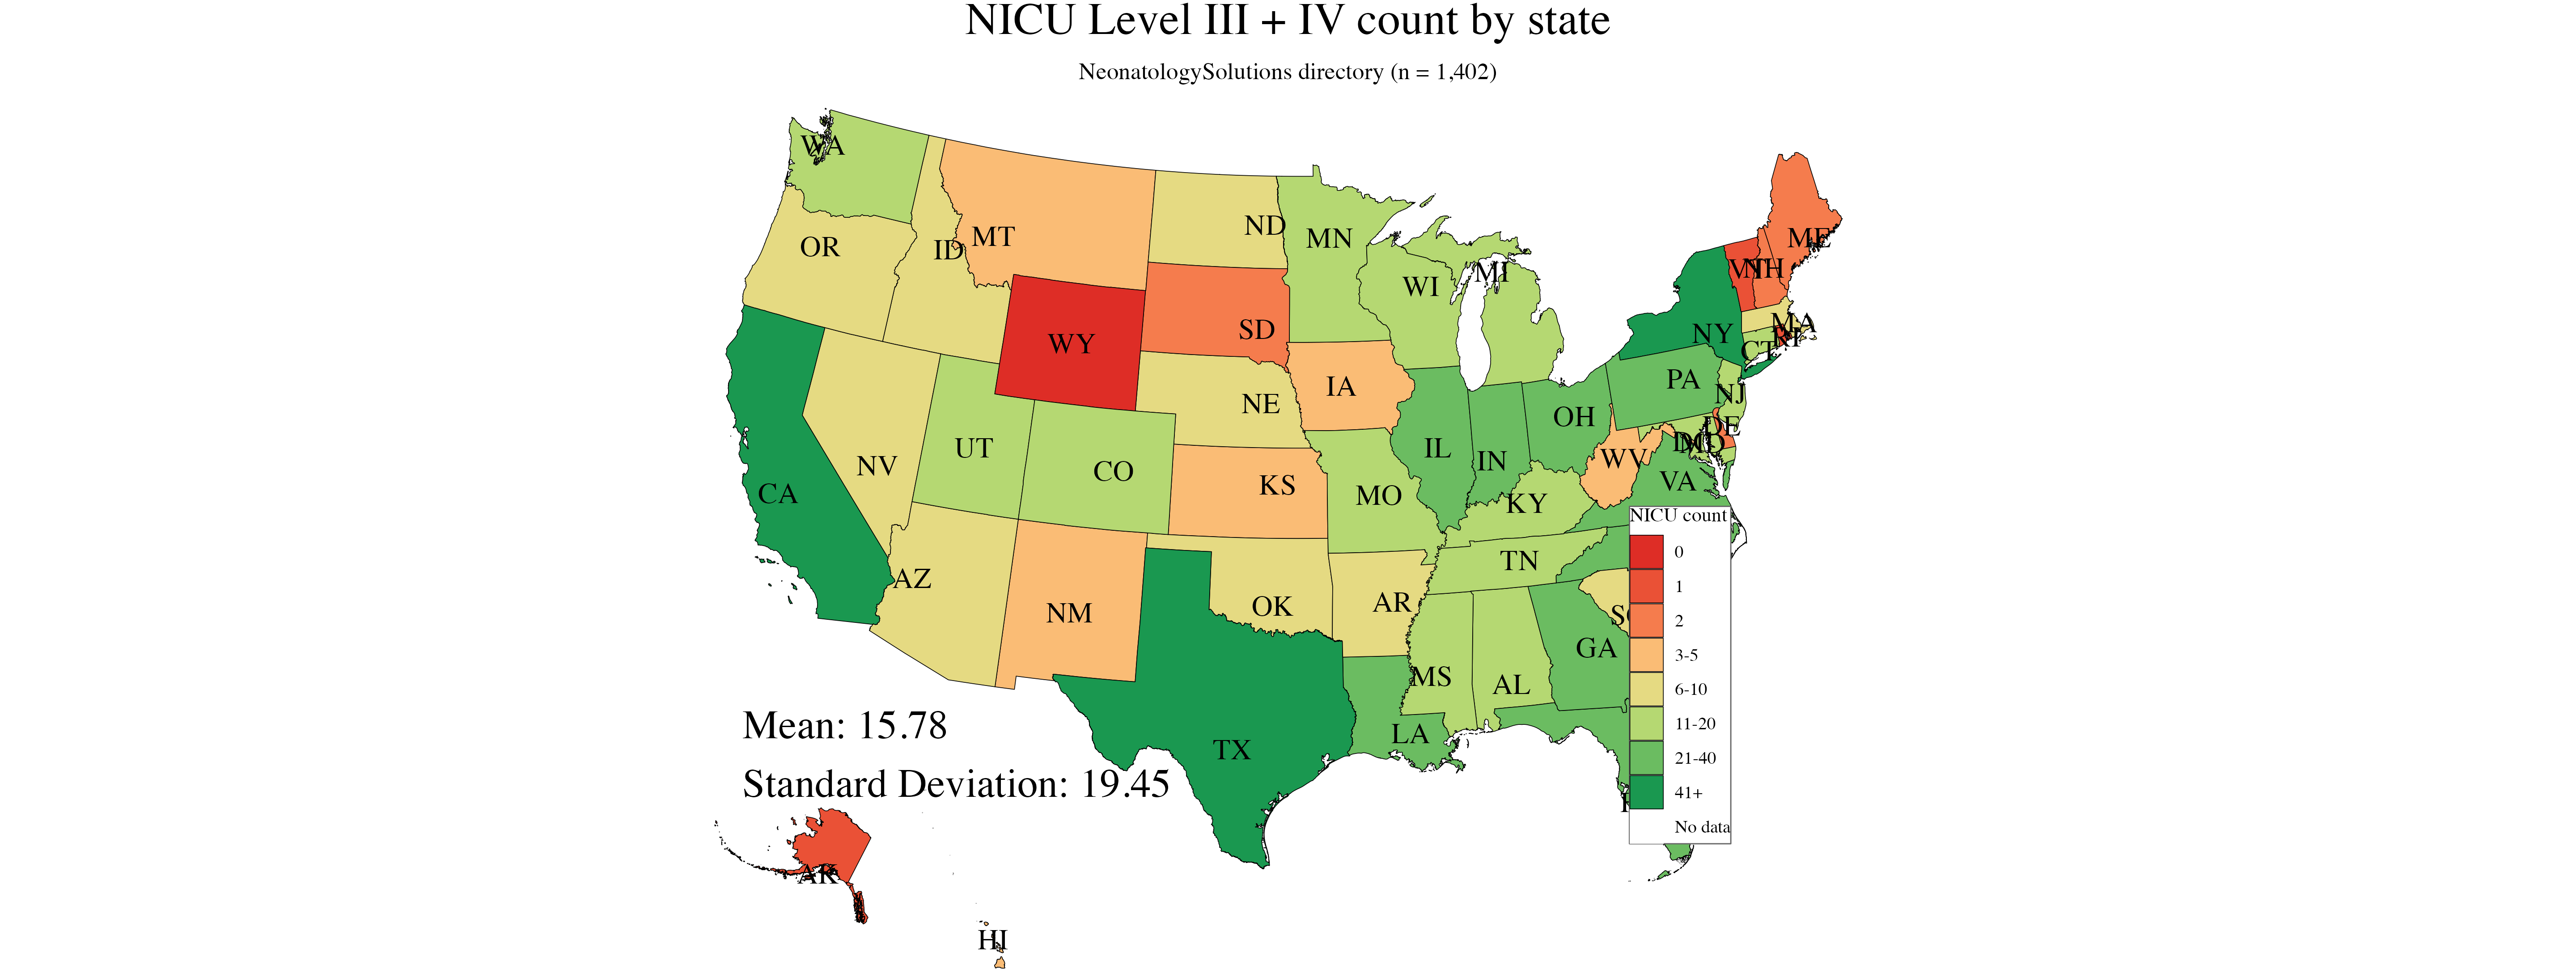
\includegraphics[width=\textwidth]{Figures/Background/nicu_state_level_III_IV_count.png}
\label{fig:nicu_state_level34_count}
\end{figure}

\begin{figure}[htbp!]
\centering
\caption{NICU Level II facility count by county}
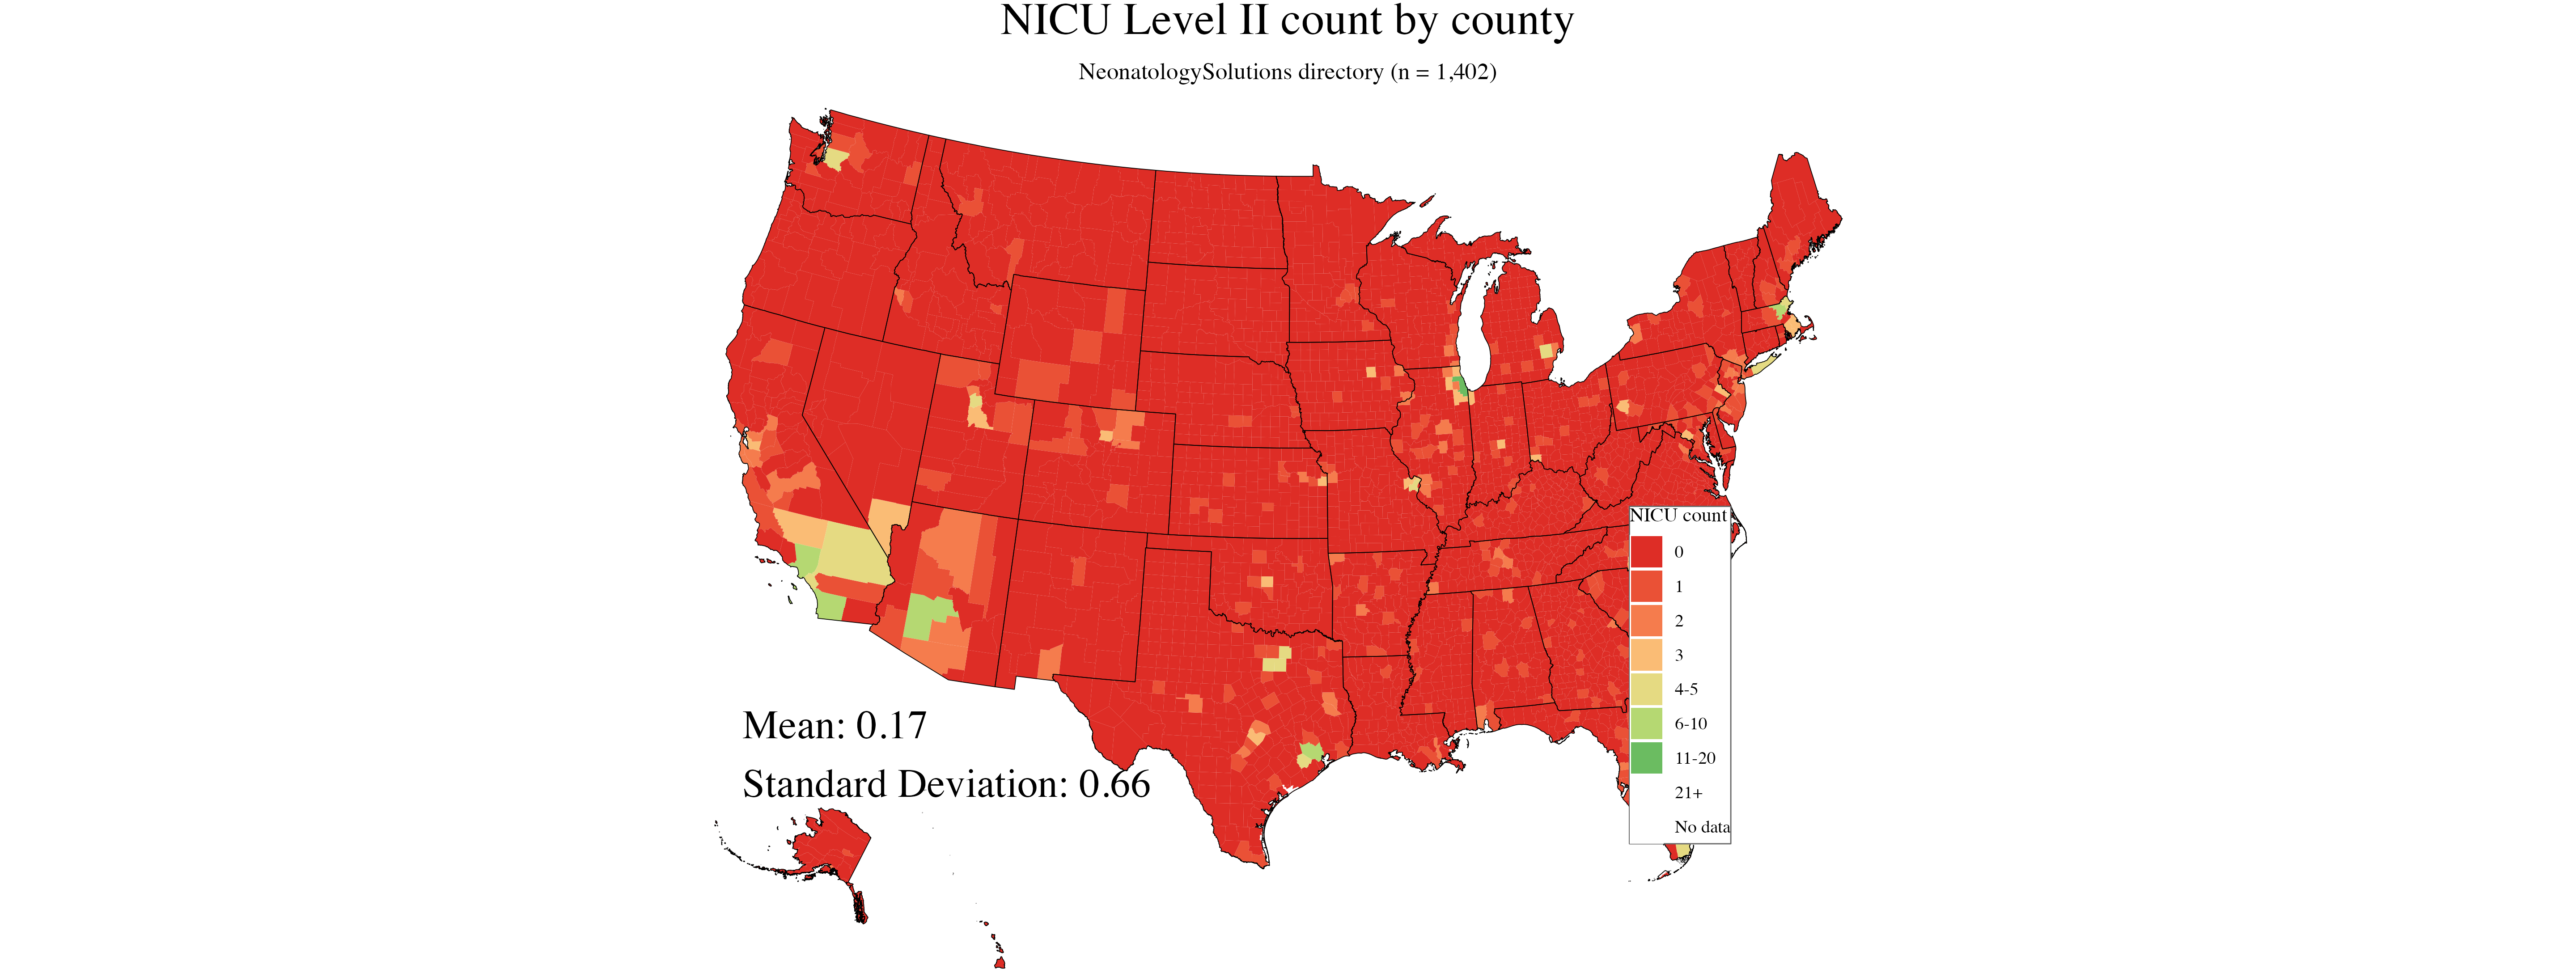
\includegraphics[width=\textwidth]{Figures/Background/nicu_county_level_II_count.png}
\label{fig:nicu_county_level2_count}
\end{figure}

\begin{figure}[htbp!]
\centering
\caption{NICU Level III + IV facility count by county}
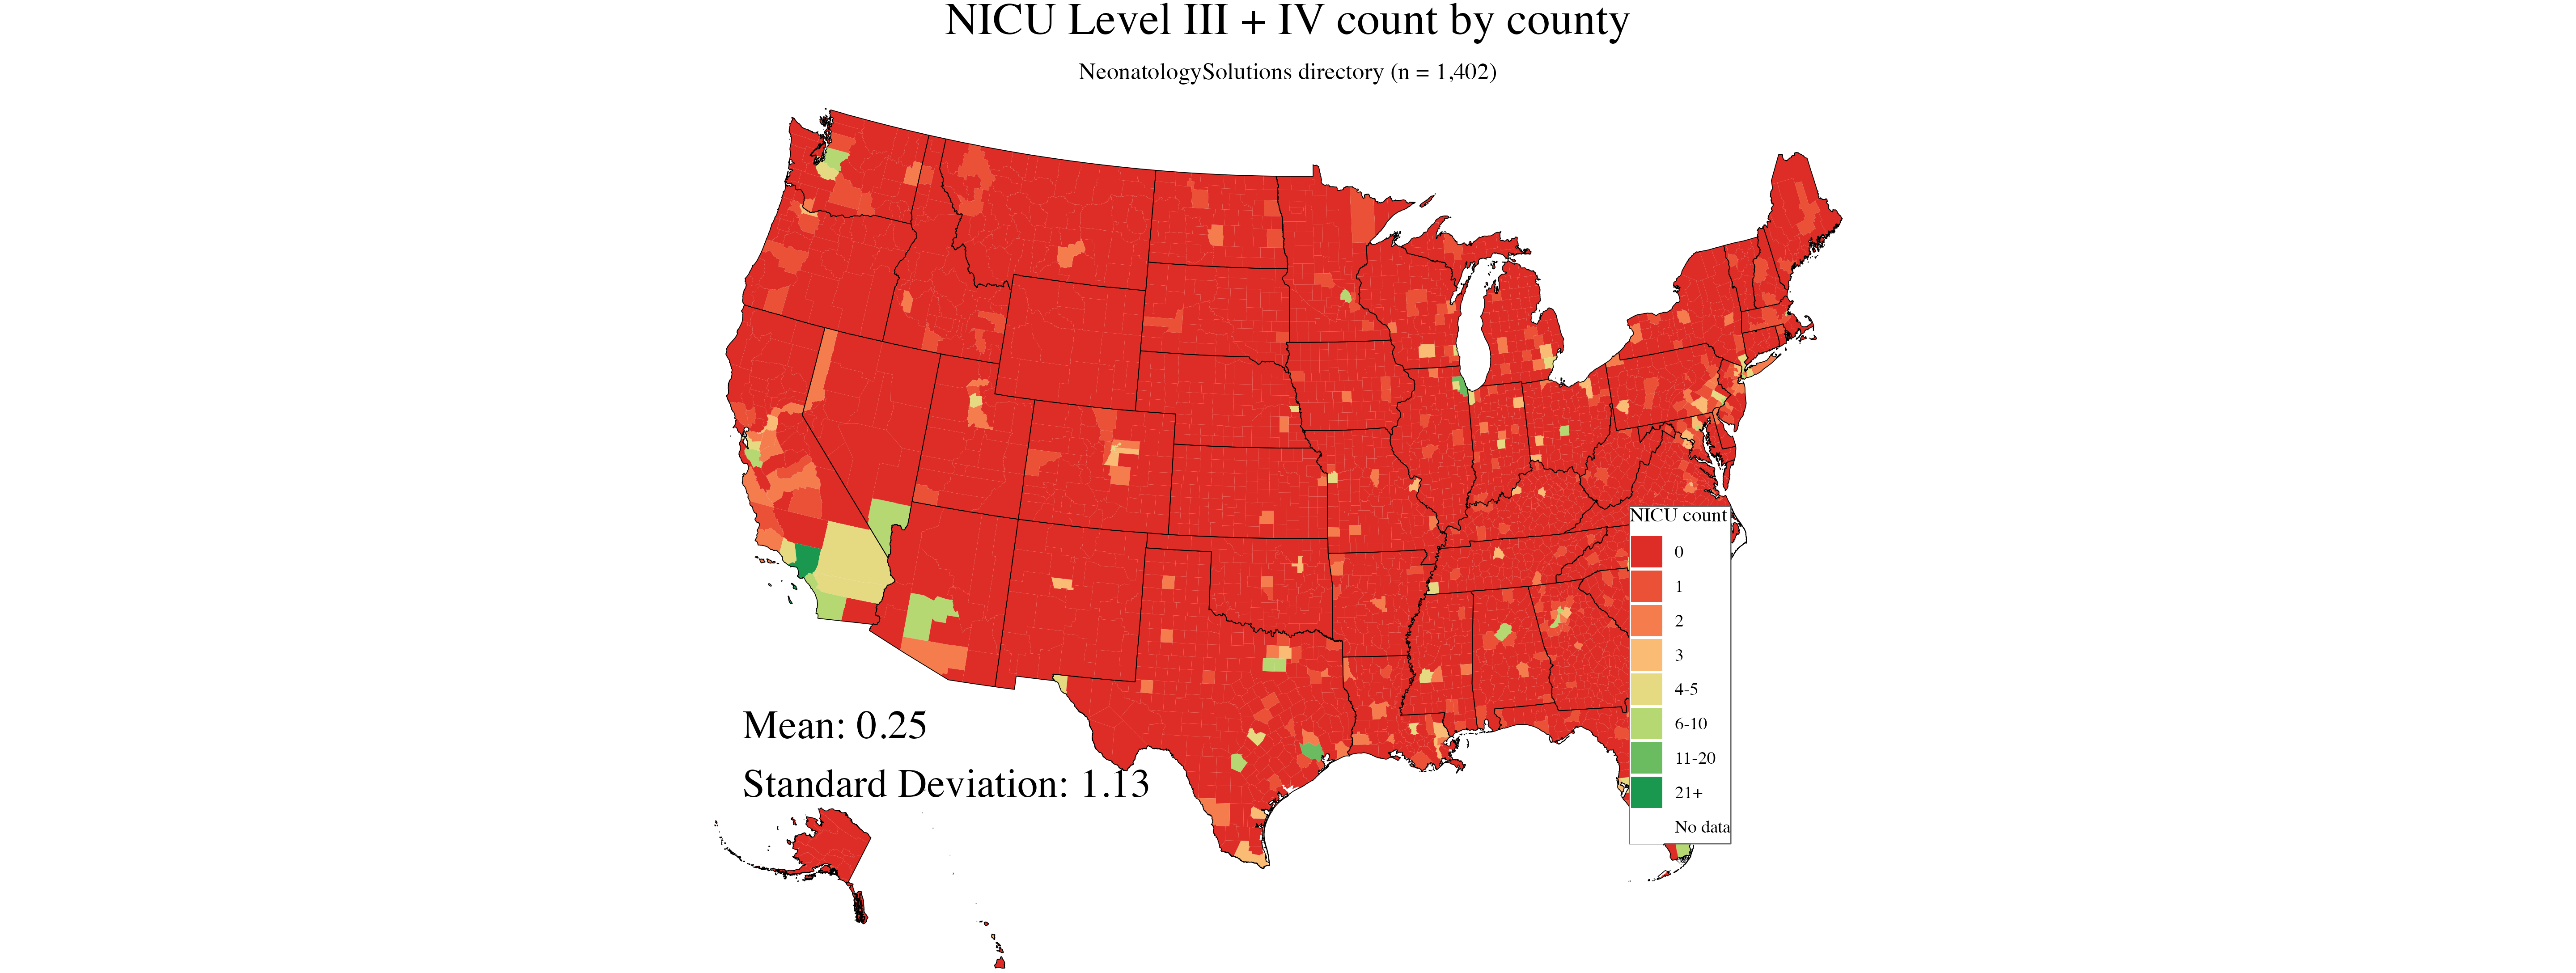
\includegraphics[width=\textwidth]{Figures/Background/nicu_county_level_III_IV_count.png}
\label{fig:nicu_county_level34_count}
\end{figure}

\begin{figure}[htbp!]
\centering
\caption{Aggregate NICU bed capacity (Level III + Level IV) by state}
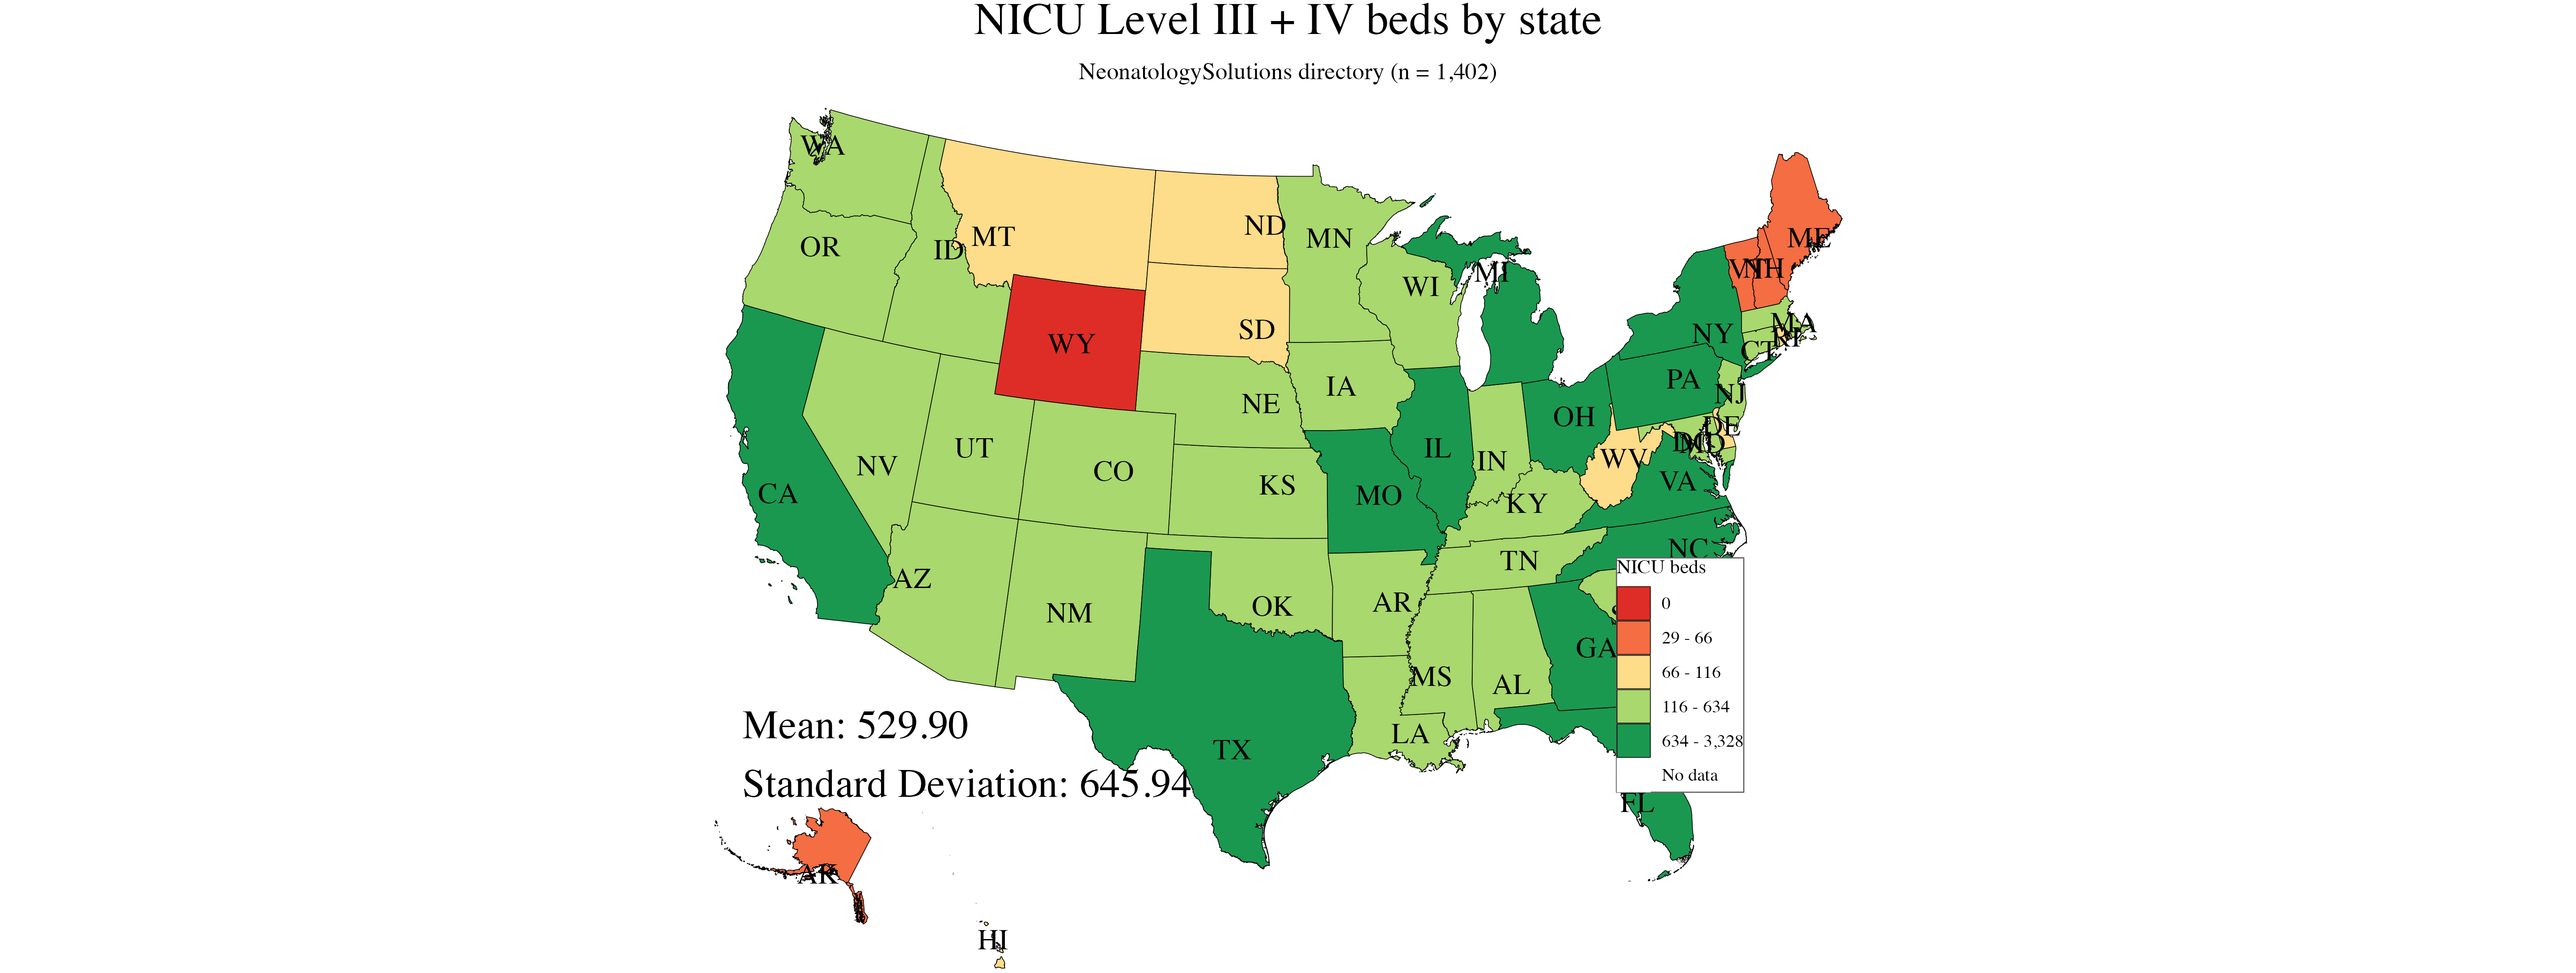
\includegraphics[width=\textwidth]{Figures/Background/nicu_state_level_III_IV_beds.png}
\label{fig:nicu_state_beds_34}
\end{figure}

\begin{figure}[htbp!]
\centering
\caption{Aggregate NICU bed capacity (Level III + Level IV) by county}
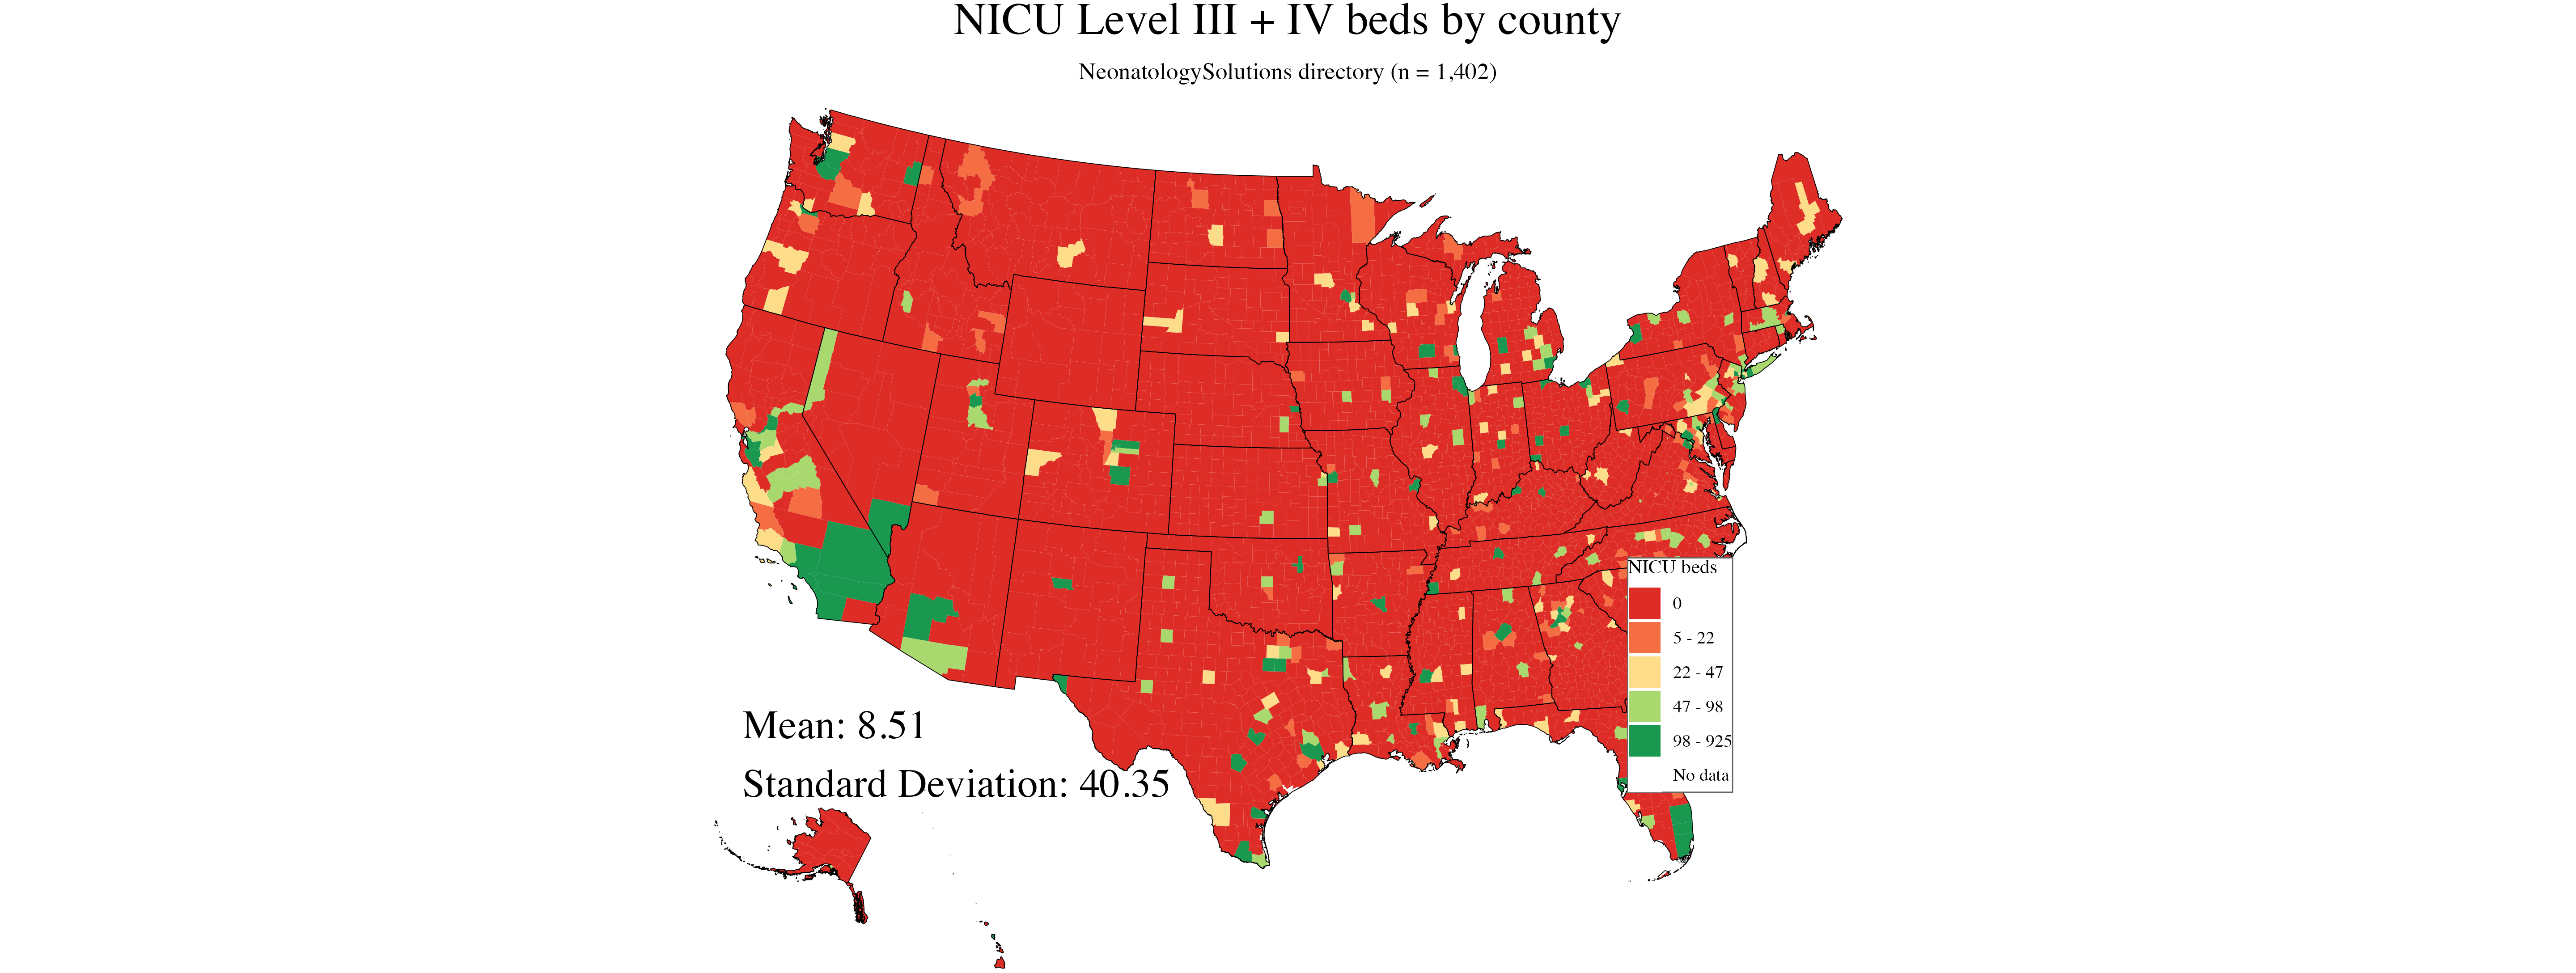
\includegraphics[width=\textwidth]{Figures/Background/nicu_county_level_III_IV_beds.png}
\label{fig:nicu_county_beds_34}
\end{figure}

\subsection{Main estimates}
We report estimates for multiple outcome definitions (diagnoses, services, medications) and multiple vulnerability tiers (preterm; low birthweight; VLBW; extreme prematurity).

\subsection{Robustness and extensions}
We assess robustness to:
(i) alternative geographic units (ZIP vs county),
(ii) alternative access definitions (nearest within 30/60/90 miles; capacity thresholds),
(iii) postpartum enrollment censoring (continuous enrollment and/or inverse probability weighting),
and (iv) within-mother designs where feasible (multiple births).

\section{Discussion}
We interpret findings in light of mechanisms (emergent transfers, travel burden, separation, care coordination), equity implications, and policy relevance (regionalization, perinatal networks, transport systems, postpartum behavioral health supports). We discuss limitations, including claims under-ascertainment of mental health and potential selection into delivery facilities.

\section*{References (placeholders)}
\begin{thebibliography}{99}
\bibitem[AAP(2012)]{AAP2012}
American Academy of Pediatrics Committee on Fetus and Newborn (2012).
\newblock Levels of Neonatal Care.
\newblock \emph{Pediatrics}, 130(3):587--597.

\bibitem[Martin et al.(2025)]{Martin2025NICU}
Martin, J.~A. et al. (2025).
\newblock Increases in Neonatal Intensive Care Admissions in the United States, 2016--2023.
\newblock NCHS Data Brief (National Vital Statistics System natality).

\bibitem[Pineda et al.(2023)]{Pineda2023Beds}
Pineda, R. et al. (2023).
\newblock NICUs in the US: levels of acuity, number of beds, and relationships to population factors.
\newblock \emph{Journal of Perinatology}.
\end{thebibliography}

\end{document}
